\documentclass[12pt,fleqn]{article}\usepackage{../common}
\begin{document}
Kisitli Boltzmann Makinalari (Restricted Boltzmann Machines -RBM-)

RBM aynen Boltzman Makinalarinda (BM) orneginde oldugu gibi bir
dagilimdir. Verilen $x,h$ icin bir olasilik degeri geri dondurebilir.
$$ p(x,h;W) = \exp (-E(x,h)) / Z $$

Standart RBM icin $h,x$ ikiseldir (binary). Gizli (hidden) tabaka $h$, ve
``gorunen (visible)'' tabaka $x$ vardir. $Z$ aynen once gordugumuz BM'de
oldugu gibi normalizasyon sabitidir. Spesifik bir RBM'i tanimlayan sey onun
$W$ matrisidir. Gizli degiskenler bazen karisiklik yaratabiliyor, bu
degiskenler aynen gorunen degiskenler gibi degiskendirler. Yani belli
$h$'lerin ``olasiligi'' sorulabilir, ya da onlar uretilebilir. Fakat RBM'i
egitirken sadece gorunen kismi tarafindan egitiriz. Gizli tabaka bu sirada
orneklem ile arada sirada ici doldurulur, bu tabii ki $W$'ye bagli olarak
yapilacaktir. Gizli tabaka daha dusuk boyutlu oldugu, ve 0/1 degerlerine
sahip olmasi mecbur oldugu icin bu git/gel bir tur ozetleme yapar ki
ogrenim bu sirada ortaya cikar.

Devam edelim, $E$ tanimina ``enerji'' olarak ta atif yapilabiliyor.

$$ E(x,h) = -h^TWx - c^Tx - b^Th $$

BM'lerden farkli olarak RBM'de $c,b$ degiskenleri var. Bu degiskenler
yanlilik (bias) icin, yani veri icindeki genel egilimi saptamalari icin
modele konulmustur. Ayrica $h^TWx$ terimi var, bu BM'deki $x^TWx$'den biraz
farkli, daha once belirttigimiz gibi, $h$ uzerinden $x$'ler arasinda
baglanti yapiyor. BM ile tum $x$ ogeleri birbirine baglanabiliyordu, RBM
ile $h$ katmaninda baglantilar paylasiliyor. Bu $h$ uzerinden baglanti
zorunlulugu RBM'in ozetleme alanini azaltarak bir tur genellemeyi
gerceklestirebiliyor. Bu yuzden onlara ``kisitli'' Boltzmann makinalari adi
veriliyor. Gizli degiskenlerin kendi aralarinda, ve gorunen degiskenlerin
kendi aralarinda direk baglantiya izin verilmemistir, ki bu daha once
bahsedilen kisitlamanin bir diger yonu. Baglantilara, $W$ uzerinden sadece
gizli ve gorunen degiskenler (tabakalar) arasinda izin verilmistir. Bu
ayrica matematiksel olarak bazi kolayliklar sagliyor, bu konuyu birazdan
isleyecegiz.

Formul alttaki gibi de acilabilir,

$$ = - \sum_j \sum_k W_{j,k}h_jx_k - \sum_k c_kx_k - \sum_j b_jh_j  $$

RBM'lerin alttaki gibi resmedildigini gorebilirsiniz.

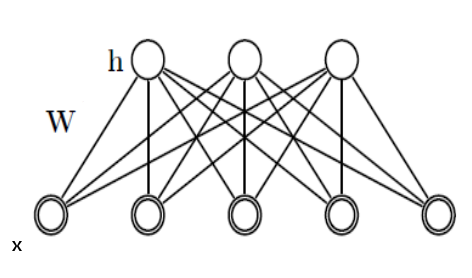
\includegraphics[height=4cm]{rbm_01.png}
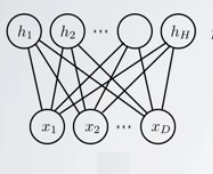
\includegraphics[height=4cm]{rbm_02.png}

Tekrar vurgulayalim, $h,x$ degiskenleri olasilik teorisinden bilinen
rasgele degiskenlerdir, yani hem $x$'e hem de $h$'e ``zar attirabiliriz'' /
bu degiskenler uzerinden orneklem toplayabiliriz.

Ayrica, RBM'ler aynen BM'ler gibi bir olasilik yogunluk fonksiyonu
uzerinden tanimlanirlar, onceki formulde gordugumuz gibi, tum mumkun
degerleri uzerinden entegralleri (ya da toplamlari) alininca sonuc 1 olur,
vs.

Devam edelim, ana formulden hareketle cebirsel olarak sunlar da dogrudur,

$$ p(x,h;W) = \exp (-E(x,h)) / Z $$

$$ 
\mlabel{2}
= \exp (h^TWx + c^Tx + b^Th ) / Z $$

$$ = \exp (h^TWx) \exp (c^Tx) \exp(b^Th) / Z $$

cunku bir toplam uzerindeki $\exp$, ayri ayri $\exp$'lerin carpimi
olur. Ayni mantikla, eger ana formulu matris / vektor yerine ayri
degiskenler olarak gormek istersek,

$$ 
p(x,h;W) = \frac{1}{Z}
\prod_j \prod_k \exp (W_{jk}h_jx_k) \prod_k \exp(c_kx_k) \prod_j \exp(b_jh_j) 
 $$

Notasyonu kolaylastirmak amaciyla $b,c$ terimlerini $W$ icine absorbe
edebiliriz, $x_0=1$ ve $h_0=1$ degerlerini mecbur tutarsak ve $w_{0,:}=c$
ve $w_{:,0}=b$ dersek, yani $W$'nin sifirinci satirinin tamaminin $c$
oldugunu, sifirinci kolonunun tamaminin $b$ oldugunu kabul edersek
RBM ana formulunu tekrar elde etmis oluruz, fakat artik

$$ E(x,h) = -h^TWx $$


$$ = - \sum_j \sum_k W_{j,k}h_jx_k  $$

ve

$$ p(x,h;W)  = \exp (h^TWx) / Z $$

yeterli olacaktir. Bir diger kolaylik $x,h$ yerine tek degisken kullanmak,

Eger $y \equiv (x,h)$ olarak alirsak ($\equiv$ tabiri ``tanim'' anlamina gelir), 


$$ P(x,h;W) = \frac{1}{Z(W)} \exp 
\bigg[ 
\frac{1}{2} y^T W y
\bigg]
$$

Aslinda acik konusmak gerekirse ``enerji'' gibi kavramlarla ugrasmak, ya da
icinde eksi terimler iceren bir grup degiskenin tekrar eksisini almak ve
eksilerin etkisini notralize etmis olmaya gerek yok, bunun yerine bastan
(2)'deki ifadeyle yola cikmak daha kisa olur. Icinde enerji olan
aciklamalari biraz da literaturde gorulebilecek anlatimlara aciklik
getirmek icin yaptik.

Simdi $h$ uzerinden marjinalize edersek,

$$ P(x;W) = \sum_h \frac{1}{Z(W)} \exp 
\bigg[ 
\frac{1}{2} y^T W y
\bigg]
$$


$$  
\mlabel{1}
P(x;W) = \frac{1}{Z(W)}  \sum_h \exp 
\bigg[ 
\frac{1}{2} y^T W y
\bigg]
$$


Ve $Z(W)$ 

$$ Z(W) = \sum_{h,x} \exp 
\bigg[ 
\frac{1}{2} y^T W y
\bigg]
$$

(1) denkleminde bolumunden sonraki kisma $Z_x(W)$ dersek, sanki ayni $\exp$
denkleminin $x$'ler uzerinden marjinalize edilmis hali olarak
gosterebiliriz onu, ve boylece daha kisa bir formul kullanabiliriz,

$$  
P(x;W) = \frac{1}{Z(W)}  
\underbrace{
\sum_h \exp 
\bigg[ 
\frac{1}{2} y^T W y
\bigg]
}_{Z_x(W)}
$$

O zaman 

$$  
P(x;W) = \frac{Z_x(W)}{Z(W)} 
$$

elde ederiz. Veri uzerinden maksimum olurluk icin, yine log uzerinden bir
hesap yapariz, BM icin yapmistik bunu,

$$  
\mathcal{L} = 
\ln \big( \prod_{n=1}^{N} P(x^{n};W) \big) = 
\sum_{n=1}^{N} \ln P(x^{n};W) 
$$

$$ 
= \sum_{n=1}^{N} \ln \frac{Z_{x^{(n)}}(W)}{Z(W)}  
= \sum_{n=1}^{N}  \big(\ln Z_{x^{(n)}} - \ln Z \big) 
$$

$$ 
\mlabel{3}
\frac{\partial \mathcal{L} }{\partial w_{ij}} = 
\sum_{n=1}^{N}  \big( \frac{\partial \ln Z_{x^{(n)}} }{\partial w_{ij}}
- \frac{\partial \ln Z }{\partial w_{ij}} \big)
$$

Parantez icindeki 1. turevi alalim,

$$ 
\frac{\partial \ln Z_{x^{(n)}} }{\partial w_{ij}} = 
\frac{\partial }{\partial w_{ij}}  
\ln \bigg[ 
\sum_h \exp \big( \frac{1}{2} y^{n^T} W y^n \big) 
\bigg]
$$

$$ 
= \frac{1}{Z_{x^{(n)}}}  \bigg[ \sum_h \frac{\partial }{\partial w_{ij}} \exp \big( \frac{1}{2} y^{n^T} W y^n  \big) \bigg]
$$

$$ 
= \frac{1}{Z_{x^{(n)}}}  
\bigg[ 
\sum_h  \exp \big( \frac{1}{2} y^{n^T} W y^n  \big) 
\frac{\partial }{\partial w_{ij}} y^{n^T} W y^n 
\bigg]
$$

$$ 
= \frac{1}{Z_{x^{(n)}}}  \sum_h  \exp \big( \frac{1}{2} y^{n^T} W y^n  \big) y_iy_j
$$


$$ 
= \sum_h  \frac{1}{Z_{x^{(n)}}}  \exp \big( \frac{1}{2} y^{n^T} W y^n  \big) y_iy_j
$$

$Z_{x^{(n)}}$'nin ne oldugunu hatirlarsak, $\exp$ ifadesinin $h$ uzerinden
marjinalize edilmis hali,

$$ 
= \sum_h  \frac{\exp \big( \frac{1}{2} y^{n^T} W y^n  \big)}
{\sum_h \exp \big( \frac{1}{2} y^T W y \big) } 
y_iy_j
$$

Eger bolumun ustunu ve altini $Z$ ile bolsek,

$$ 
= \sum_h  
\frac{\exp \big( \frac{1}{2} y^{n^T} W y^n  \big) / Z} 
{\sum_h \exp \big( \frac{1}{2} y^T W y \big) / Z} 
y_iy_j
$$

Ust kisim $P(y;W)$ yani $P(x,h;W) $ alt kisim $P(x;W)$ olmaz mi? Evet! Ve,


$$ P(h|x^n;W) = \frac{P(x^n,h;W)}{P(x^n;W)}  $$

olduguna gore, 

$$ =  \sum_h P(h|x^n;W) y_iy_j $$

elde ederiz. Bunu da $<y_iy_j>_{P(h|x^n;W)}$ olarak yazabiliriz. 

Simdi parantez icindeki 2. turevi alalim, yani $\frac{\partial \ln Z }{\partial w_{ij}} $,

$$ 
\frac{\partial \ln Z }{\partial w_{ij}}  = 
\sum_{h,x} \frac{1}{Z}  \exp \big( \frac{1}{2} y^{T} W y  \big) y_iy_j =
\sum_{h,x} P(y;W)  y_iy_j
$$

ki bu son ifadeyi de $<y_iy_j>_{P(y;W)}$ olarak yazabiliriz. Tamamini,
yani (3) ifadesini, artik soyle yazabiliriz,

$$
\mlabel{4}
\sum_{n=1}^{N}  \big( \frac{\partial \ln Z_{x^{(n)}} }{\partial w_{ij}} - \frac{\partial \ln Z }{\partial w_{ij}} \big)
= \sum_{n=1}^{N}  <y_iy_j>_{P(h|x^n;W)} - <y_iy_j>_{P(y;W)}
$$

Bu formulu de BM icin yaptigimiz gibi bir gradyan guncelleme formulune
donusturebiliriz. Guncelleme formulunun hangi hesaplari gerektirdigine
gelince; Ilk terim tum $h$'ler uzerinden, ikincisi ise tum $x,h$'ler
uzerinden bir olasilik hesabi ve ornekleme gerektirecek. Bu durum cetin
hesap (intractable) denen bir durum, ozellikle $x,h$ sarti icin; daha once
BM icin bu problemi Gibbs orneklemesi ile cozmustuk. Ayni cozumu burada da
uygulayabiliriz, fakat belki daha iyi bir yaklasim su olacak.

CD Yontemi (Contrastive Divergence) 

RBM'leri egitmek icin kullanilan en populer yontem CD yontemidir. Bu
teknigi anlatmadan once bazi matematiksel kolayliklari bilmek gerekli.

RBM grafigine bakarsak, eger $x$ biliniyor ise bu $h$ degiskenlerini
bagimsiz hale getirir (kosullu olasilik kurali), ve ayni sekilde $h$
biliniyor ise $x$ bagimsiz hale gelir. Bunu gorsel olarak bile anlamak cok
kolay, elimizle tum $x$'leri kapatalim mesela ve $h$ dugumlerine bakalim,
aralarinda hicbir baglanti yoktur degil mi? Ayni sekilde $h$ kapatinca
$x$'ler ``baglantisiz'' hale gelir. 

Bu bagimsizliktan yola cikarak, daha once BM icin yaptigimiz gibi,
olasiliklar su basit formullere donusur,

$$ P(h_i=1|x) = \sigma \bigg( \sum _{j=1}^{m} w_{ij} x_j \bigg) $$

$$ P(x_i=1|h) = \sigma \bigg( \sum _{i=1}^{n} w_{ij} h_i \bigg) $$

ve tabii ki $\sigma(x) = 1 / (1+e^{-x})$. Daha once 1 olma olasiligini
nasil ornekleme cevirecegimizi de gormustuk zaten. 

Simdi CD'nin ne olduguna gelelim. Eger RBM icin gereken orneklemeyi klasik
Gibbs ile yaparsak ornekleme zincirini ``yeterince uzun sure'' isletmek
gerekir ki dagilimin olasi noktalari gezilmis olsun. Fakat, ozellikle
yuksek boyutlu durumlarda, tum $x,h$ kombinasyonlarini dusunursek bu cok
buyuk bir alandir ve gezme islemi cok, cok uzun zaman alabilir. Bunun
yerine, ve ustteki bagimsizlik formullerinden hareketle CD yontemi
bulunmustur, bu yonteme gore ornekleme verinin {\em kendisinden} baslatilir
(kiyasla pur Gibbs rasgele bir noktadan), dongunun mesela ilk adiminda
$x^0$ (ki bu tum verinin tamami), baz alinarak $p(h^0|v^0)$ hesaplanir
(ustteki sigmoid), onun uzerinden $h^0$ orneklemi alinir, sonra $h^0$ baz
alinir ve $x^1$ uretilir, bu boyle devam eder. Boylece mumkun $h$ ve
$x$'ler gezilmis olur. Not: Surekli verinin kendisine donmenin de bazi
dezavantajlari var, ki bunu yapmadan pur Gibbs orneklemesine daha yakin bir
yaklasim Kalici (Persistent) CD adli yontemdir (tabii baska yaklasiksal
numaralar kullanarak).

Literaturde su sekildeki resim bolca gorulebilir,

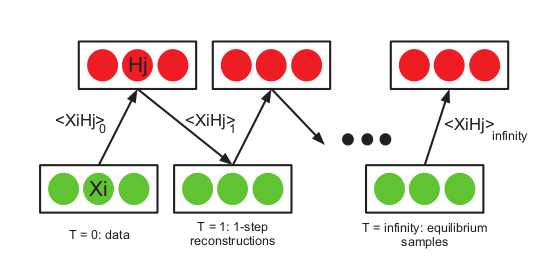
\includegraphics[height=5cm]{rbm_03.png}

Bu yontem pur Gibbs orneklemesine kiyasla cok daha hizli isler ve iyi
sonuclar verir. Teorik olarak niye isledigi [1,2,4] makalelerinde
bulunabilir. CD aslinda (4) hedef formulunu degil baska bir hedefi optimize
ediyor, fakat sonuc orijinal gradyan adimlarinin yapmak istedigine
yakin. [3] baz alinarak, su sekilde kodlanabilir,

\inputminted[fontsize=\footnotesize]{python}{rbm.py}

RBM ve Siniflama 

Siniflama (classification) islemi yapmak icin BM orneginde bir
normalizasyon sabiti hesaplamistik. Burada degisik bir yoldan gidecegiz; ki
bu yol ileride Derin Ogrenim icin faydali olacak. 

Egittikten sonra bir RBM, icindeki $W$'ye gore, herhangi bir ``gorunur''
veri noktasi $x$ icin bir gizli bir $h$ uretebilir. Bunu ustteki
formulasyondan zaten biliyoruz. Ayrica, $h$ genellikle daha az boyutta
olduguna gore (hatta olmasa bile) bu $h$ uretiminin bir tur transformasyon
oldugu, veri uzerinde bir ``ozetleme'' yaptigi iddia edilebilir. O zaman
teorik olarak, gorunur veri yerine, gorunur veriden uretilen gizli veriyi
kullanirsak ve bu veriyi alip baska bir siniflayiciya verirsek, mesela
lojistik regresyon gibi, bu $h$'ler ve etiketler uzerinden takip edilen bir
(supervised) egitim yapabiliriz. Yani, once RBM egitiyoruz, tum verinin $h$
karsiligini aliyoruz, sonra bunlari lojistik regresyona veriyoruz. Alttaki
kodda bunun orneginin gorebiliriz.

Bu kod, ayrica, k-Katlama (k-fold) teknigini uyguluyor, veriyi 3 parcaya
bolup sirasiyla tum parcalari birer kez test, digerlerini egitim verisi
yapiyor, boylece verinin tamami uzerinden egitim/test yapmis
olunuyor. Sonuc,

\inputminted[fontsize=\footnotesize]{python}{test_rbmkfold.py}

\begin{minted}[fontsize=\footnotesize]{python}
! python test_rbmkfold.py
\end{minted}

\begin{verbatim}
1.0
\end{verbatim}

Basari yuzde 100! Altta karsilastirma icin KNN teknigi kullandik,

\inputminted[fontsize=\footnotesize]{python}{test_knnkfold.py}

\begin{minted}[fontsize=\footnotesize]{python}
! python test_knnkfold.py
\end{minted}

\begin{verbatim}
0.98009506833
\end{verbatim}

Kaynaklar

[1] Hinton, G., {\em Training Products of Experts by Minimizing Contrastive
Divergence}

[2] Louppe, G., {\em Collaborative filtering, Scalable approaches using
restricted Boltzmann machines}, Master Tezi, 2010

[3] \url{https://github.com/echen/restricted-boltzmann-machines}

[4] Tieleman, Hinton, {\em Using Fast Weights to Improve Persistent Contrastive Divergence}



\end{document}
